\documentclass[12pt]{article}
\usepackage[left=1cm, right=1cm, top=2cm,bottom=1.5cm]{geometry} 

\usepackage[parfill]{parskip}
\usepackage[utf8]{inputenc}
\usepackage[T2A]{fontenc}
\usepackage[russian]{babel}
\usepackage{enumitem}
\usepackage[normalem]{ulem}
\usepackage{amsfonts, amsmath, amsthm, amssymb, mathtools,xcolor,accents}
\usepackage{blkarray}

\usepackage{tabularx}
\usepackage{hhline}

\usepackage{accents}
\usepackage{fancyhdr}
\pagestyle{fancy}
\renewcommand{\headrulewidth}{1.5pt}
\renewcommand{\footrulewidth}{1pt}

\usepackage{graphicx}
\usepackage[figurename=Рис.]{caption}
\usepackage{subcaption}
\usepackage{float}

%%Наименование папки откуда забирать изображения
\graphicspath{ {./images/} }

%%Изменение формата для ввода доказательства
\renewcommand{\proofname}{$\square$  \nopunct}
\renewcommand\qedsymbol{$\blacksquare$}

%%Изменение отступа на таблицах
\addto\captionsrussian{%
	\renewcommand{\proofname}{$\square$ \nopunct}%
}
%% Римские цифры
\newcommand{\RN}[1]{%
	\textup{\uppercase\expandafter{\romannumeral#1}}%
}

%% Для удобства записи
\newcommand{\MR}{\mathbb{R}}
\newcommand{\MC}{\mathbb{C}}
\newcommand{\MQ}{\mathbb{Q}}
\newcommand{\MN}{\mathbb{N}}
\newcommand{\MZ}{\mathbb{Z}}
\newcommand{\MTB}{\mathbb{T}}
\newcommand{\MTI}{\mathbb{I}}
\newcommand{\MI}{\mathrm{I}}
\newcommand{\MCI}{\mathcal{I}}
\newcommand{\MJ}{\mathrm{J}}
\newcommand{\MH}{\mathrm{H}}
\newcommand{\MT}{\mathrm{T}}
\newcommand{\MU}{\mathcal{U}}
\newcommand{\MV}{\mathcal{V}}
\newcommand{\MB}{\mathcal{B}}
\newcommand{\MF}{\mathcal{F}}
\newcommand{\MW}{\mathcal{W}}
\newcommand{\ML}{\mathcal{L}}
\newcommand{\MP}{\mathcal{P}}
\newcommand{\VN}{\varnothing}
\newcommand{\VE}{\varepsilon}
\newcommand{\dx}{\, dx}
\newcommand{\dy}{\, dy}
\newcommand{\dz}{\, dz}
\newcommand{\dd}{\, d}


\theoremstyle{definition}
\newtheorem{defn}{Опр:}
\newtheorem{rem}{Rm:}
\newtheorem{prop}{Утв.}
\newtheorem{exrc}{Упр.}
\newtheorem{problem}{Задача}
\newtheorem{lemma}{Лемма}
\newtheorem{theorem}{Теорема}
\newtheorem{corollary}{Следствие}

\newenvironment{cusdefn}[1]
{\renewcommand\thedefn{#1}\defn}
{\enddefn}

\DeclareRobustCommand{\divby}{%
	\mathrel{\text{\vbox{\baselineskip.65ex\lineskiplimit0pt\hbox{.}\hbox{.}\hbox{.}}}}%
}
\DeclareRobustCommand{\ndivby}{\mkern-1mu\not\mathrel{\mkern4.5mu\divby}\mkern1mu}


%Короткий минус
\DeclareMathSymbol{\SMN}{\mathbin}{AMSa}{"39}
%Длинная шапка
\newcommand{\overbar}[1]{\mkern 1.5mu\overline{\mkern-1.5mu#1\mkern-1.5mu}\mkern 1.5mu}
%Функция знака
\DeclareMathOperator{\sgn}{sgn}

%Функция ранга
\DeclareMathOperator{\rk}{\text{rk}}
\DeclareMathOperator{\diam}{\text{diam}}


%Обозначение константы
\DeclareMathOperator{\const}{\text{const}}

\DeclareMathOperator{\codim}{\text{codim}}

\DeclareMathOperator*{\dsum}{\displaystyle\sum}
\newcommand{\ddsum}[2]{\displaystyle\sum\limits_{#1}^{#2}}
\newcommand{\ddssum}[2]{\displaystyle\smashoperator{\sum\limits_{#1}^{#2}}}
\newcommand{\ddlsum}[2]{\displaystyle\smashoperator[l]{\sum\limits_{#1}^{#2}}}
\newcommand{\ddrsum}[2]{\displaystyle\smashoperator[r]{\sum\limits_{#1}^{#2}}}

%Интеграл в большом формате
\DeclareMathOperator{\dint}{\displaystyle\int}
\newcommand{\ddint}[2]{\displaystyle\int\limits_{#1}^{#2}}
\newcommand{\ssum}[1]{\displaystyle \sum\limits_{n=1}^{\infty}{#1}_n}

\newcommand{\smallerrel}[1]{\mathrel{\mathpalette\smallerrelaux{#1}}}
\newcommand{\smallerrelaux}[2]{\raisebox{.1ex}{\scalebox{.75}{$#1#2$}}}

\newcommand{\smallin}{\smallerrel{\in}}
\newcommand{\smallnotin}{\smallerrel{\notin}}

\newcommand*{\medcap}{\mathbin{\scalebox{1.25}{\ensuremath{\cap}}}}%
\newcommand*{\medcup}{\mathbin{\scalebox{1.25}{\ensuremath{\cup}}}}%

\makeatletter
\newcommand{\vast}{\bBigg@{3.5}}
\newcommand{\Vast}{\bBigg@{5}}
\makeatother

%Промежуточное значение для sup\inf, поскольку они имеют разную высоту
\newcommand{\newsup}{\mathop{\smash{\mathrm{sup}}}}
\newcommand{\newinf}{\mathop{\mathrm{inf}\vphantom{\mathrm{sup}}}}

%Скалярное произведение
\newcommand{\inner}[2]{\left\langle #1, #2 \right\rangle }
\newcommand{\linsp}[1]{\left\langle #1 \right\rangle }
\newcommand{\linmer}[2]{\left\langle #1 \vert #2\right\rangle }

%Подпись символов снизу
\newcommand{\ubar}[1]{\underaccent{\bar}{#1}}

%%Шапка для букв сверху
\newcommand{\wte}[1]{\widetilde{#1}}
\newcommand{\wht}[1]{\widehat{#1}}
\newcommand{\ovl}[1]{\overline{#1}}


%%Трансформация Фурье
\newcommand{\fourt}[1]{\mathcal{F}\left(#1\right)}
\newcommand{\ifourt}[1]{\mathcal{F}^{-1}\left(#1\right)}

%%Символ вектора
\newcommand{\vecm}[1]{\overrightarrow{#1\,}}

%%Пространстов матриц
\newcommand{\matsq}[1]{\operatorname{Mat}_{#1}}
\newcommand{\mat}[2]{\operatorname{Mat}_{#1, #2}}

%Оператор для действ и мнимых чисел
\DeclareMathOperator{\IM}{\operatorname{Im}}
\DeclareMathOperator{\RE}{\operatorname{Re}}
\DeclareMathOperator{\li}{\operatorname{li}}
\DeclareMathOperator{\GL}{\operatorname{GL}}
\DeclareMathOperator{\SL}{\operatorname{SL}}
\DeclareMathOperator{\Char}{\operatorname{char}}
\DeclareMathOperator\Arg{Arg}
\DeclareMathOperator\ord{ord}

%Оператор для образа
\DeclareMathOperator{\Ima}{Im}

%Делимость чисел
\newcommand{\modn}[3]{#1 \equiv #2 \; (\bmod \; #3)}
\newcommand{\nmodn}[3]{#1 \not\equiv #2 \; (\bmod \; #3)}

%%Взятие в скобки, модули и норму
\newcommand{\parfit}[1]{\left( #1 \right)}
\newcommand{\modfit}[1]{\left| #1 \right|}
\newcommand{\sqparfit}[1]{\left\{ #1 \right\}}
\newcommand{\normfit}[1]{\left\| #1 \right\|}

%%Функция для обозначения равномерной сходимости по множеству
\newcommand{\uconv}[1]{\overset{#1}{\rightrightarrows}}
\newcommand{\uconvm}[2]{\overset{#1}{\underset{#2}{\rightrightarrows}}}

%% Функция для добавления круга сверху множества
\newcommand{\Circ}[1]{\accentset{\circ}{#1}}

%%Функция для обозначения нижнего и верхнего интегралов
\def\upint{\mathchoice%
	{\mkern13mu\overline{\vphantom{\intop}\mkern7mu}\mkern-20mu}%
	{\mkern7mu\overline{\vphantom{\intop}\mkern7mu}\mkern-14mu}%
	{\mkern7mu\overline{\vphantom{\intop}\mkern7mu}\mkern-14mu}%
	{\mkern7mu\overline{\vphantom{\intop}\mkern7mu}\mkern-14mu}%
	\int}
\def\lowint{\mkern3mu\underline{\vphantom{\intop}\mkern7mu}\mkern-10mu\int}

%%След матрицы
\DeclareMathOperator*{\tr}{tr}

\makeatletter
\renewcommand*\env@matrix[1][*\c@MaxMatrixCols c]{%
	\hskip -\arraycolsep
	\let\@ifnextchar\new@ifnextchar
	\array{#1}}
\makeatother


%% Переопределение функции хи, чтобы выглядела более приятно
\makeatletter
\@ifdefinable\@latex@chi{\let\@latex@chi\chi}
\renewcommand*\chi{{\@latex@chi\smash[t]{\mathstrut}}} % want only bottom half of \mathstrut
\makeatletter

\setcounter{MaxMatrixCols}{20}

\begin{document}
\lhead{Математический анализ - \RN{4}}
\chead{Шапошников С.В.}
\rhead{Лекция - 8}

\section*{Применение формулы замены переменной}
\subsection*{Теорема Брауэра}
\begin{theorem}(\textbf{Брауэра})
	Если $f$ - непрерывное отображение замкнутого шара: $\ovl{\MB}(0,1) \to \ovl{\MB}(0,1)$, то:
	$$
		\exists \, x_0 \in \ovl{\MB}(0,1) \colon f(x_0) = x_0
	$$
\end{theorem}
\begin{proof}(Продолжение доказательства):
	
	$f \colon \MR^n \to \MR^n$ - гладкое отображение, $f\colon \ovl{\MB} \to \ovl{\MB}$. Предположим, что $f(x) \neq x$ на $\ovl{\MB}$, тогда проведём луч через $f(x)$ и $x$ до пересечения с границей:
	$$
		F(x) = x + \lambda(x){\cdot}(x - f(x)), \quad \lambda(x) = \dfrac{-\inner{x}{x-f(x)} + \sqrt{\inner{x}{x - f(x)}^2  + (1 - \|x\|^2){\cdot}\|x - f(x)\|^2}}{\|x - f(x)\|^2}
	$$
	\begin{enumerate}[label=(\arabic*)]
		\item $F(x)$ - гладкое отображение в $\MB(0,1 + \delta), \, \delta > 0$;
		\item $\|F(x)\| = 1$, то есть: $F \colon \ovl{\MB}(0,1) \to \partial \ovl{\MB}(0,1)$;
		\item (\uline{Ретракция}): $\forall x \in \partial \MB(0,1), \, F(x) = x$;
	\end{enumerate}
	\textbf{\uline{Идея}}: Из того, что $f(x) \neq x$, мы построим такое отображение $F(x)$, а затем с помощью ФЗП поймем, что такого отображения не существует и придём к противоречию. То, что такого отображения не существует и называется леммой о барабане/леммой об отсутствии ретракции шара на свою границу. Нам надо понять, что можно сказать про подкоренное выражение:
	$$
		\psi(x) = \underbrace{\inner{x}{x - f(x)}^2}_{\geq 0}  + \underbrace{(1 - \|x\|^2)}_{\geq 0, \,\forall x \in \ovl{\MB}(0,1)}{\cdot}\underbrace{\|x - f(x)\|^2}_{\neq 0, \, \forall x \in \MB(0,1 + \delta)} \geq 0
	$$
	Мы показали, что $\psi(x) > 0$ в $\MB(0,1 + \delta)$ и таким образом, мы проверили корректность всех трех свойств, ожидаемых от функции $F(x)$.
	
	Докажем, что такого $F(x)$ не существует и придём к противоречию. Возьмем $t \in [0,1]$ и рассмотрим функцию (линейная гомотопия тождественного отображения и отображения $F$):
	$$
		F_t(x) = (1 - t)x + tF(x)
	$$
	Заметим, что $F_t(x)$ в окрестности $\MB(0,1 + \tfrac{\delta}{2})$ - гладкое отображение и $\exists \, t_0 \in (0,1) \colon \forall t \in[0,t_0]$ выполнено:
	\begin{enumerate}[label=\arabic*)]
		\item $F_t(x)$ - инъекция на $\MB(0,1 + \tfrac{\delta}{2})$;
		\item $\det{F'_t} > 0$ на окрестности $\MU \colon \ovl{\MB}(0,1) \subset \MU = \MB(0,1 + \tfrac{\delta}{2})$. Рассмотрим функцию: $(t,x) \mapsto \det{F'_t(x)}$, она непрерывна на компакте $[0,1] \times \MB(0,1 + \tfrac{\delta}{2}) \Rightarrow$ равномерно непрерывна на нём. Заметим, что $\det{F'_0(x)} = 1$ и из равномерной непрерывности верно:
		$$
			\exists \, t_0 \colon t \in [0, t_0], \, \forall x \in \ovl{\MB}(0, 1 + \tfrac{\delta}{2}), \,  |\det{F'_t(x)} - \det{F'_0(x)}| \leq \tfrac{1}{2} \Rightarrow  \forall x \in \ovl{\MB}(0, 1 + \tfrac{\delta}{2}), \, \det{F'_t(x)} \geq \tfrac{1}{2}
		$$
	\end{enumerate}
	Пусть $t \in [0, t_0]$, тогда $F_t(\MB(0,1 + \tfrac{\delta}{2}))$ - открытое множество и $F_t \colon \MB(0, 1 + \tfrac{\delta}{2}) \to F_t(\MB(0,1 + \tfrac{\delta}{2}))$ это диффеоморфизм: Возьмем шар $\MB(0, 1 + \tfrac{\delta}{2})$ и точку $a$ в нём, её образ - $F_t(a)$, матрица якоби в этой точке $F'_t(a)$ - невырождена $\Rightarrow$ по теореме об обратной функции существуют окрестности $\MV$ и $\MW$ между которыми $F_t$ устанавливает диффеоморфизм $\Rightarrow$ в образе $F'_t$ лежит образ целой окрестности из шара, следовательно $F_t(a)$ - внутренняя точка $F_t(\MB(0, 1 + \tfrac{\delta}{2}))$.
	\begin{enumerate}[label=\arabic*)]
		\item Все точки отображения внутренние $\Rightarrow$ образ это открытое множество;
		\item Отображение $F_t(x)$ инъективно, а также оно сюръективно по построению $\Rightarrow$ это биекция и локально у каждой точки в образе есть окрестность на которой обратная является диффеоморфизмом $\Rightarrow$ непрерывно дифференцируемая в обе стороны биекция $\Rightarrow$ диффеоморфизм;
	\end{enumerate}
	 Рассмотрим шар $\MB = \MB(0,1)$ - открытый шар, $\forall x \in \MB, \, \|x\| < 1$, рассмотрим его образ:
	 $$
	 	\|x\| < 1 \Rightarrow \|F_t(x)\| \leq \underbrace{(1 -t)}_{>0}{\cdot}\underbrace{\|x\|}_{< 1} + t{\cdot}\|F(x)\| = (1 - t){\cdot}\|x\| + t  < 1 - t + t < 1 \Rightarrow F_t(\MB) \subset \MB
	 $$
	 Так как $F_t$ - диффеоморфизм, то $F_t(\MB)$ - открытое множество в $\MB$. Кроме того, $F_t(\MB)$ - замкнуто в $\MB$ (индуцированная топология $\MB$): возьмем последовательность точек $y_n \in F_t(\MB) \colon y_n \to y \in \MB$ и проверим, что $y \in F_t(\MB)$. Поскольку $F_t$ - диффеоморфизм, то возьмем $x_n = F_t^{-1}(y_n) \in \MB$, тогда по непрерывности обратной функции $F_t^{-1}$ будет верно: $x_n \to x = F_t^{-1}(y)$. Если $x$ окажется на границе, тогда $\|x\| = 1 \Rightarrow$ очевидно, что: $\|x\| \leq 1$. Предположим, что $\|x\| = 1$, тогда:
	 $$
	 	\|x \| = 1 \Rightarrow F(x) = x \Rightarrow F_t(x) = (1 - t)x + tx = x \Rightarrow \|F_t(x)\| = \|x\| = 1
	 $$
	 С другой стороны, $\|F_t(x)\| =\|y\| < 1$, поскольку $y \in \MB \Rightarrow$ противоречие $\Rightarrow \|x\| < 1 \Rightarrow y \in F_t(\MB)$. Итого:
	 $$
	 	F_t(\MB) \subset \MB, \, F_t(\MB) \neq \VN, \, F_t(\MB) \text{ - открыто и замкнуто в } \MB
	 $$
	 Поскольку $\MB$ - связно, то $F_t(\MB) = \MB$, так как $F_t(\MB) \neq \VN$. Рассмотрим объем $\MB$:
	 $$
	 	|\MB| = |F_t(\MB)| \overset{\text{ФЗП}}{=} \ddint{\MB}{}\underbrace{\det{F'_t(x)}}_{ > 0}dx = P(t) \text{ - многочлен по }t
	 $$
	 где $F'_t(x) = (1 - t)\MI + tF'(x) \Rightarrow$ определитель $F'_t(x)$ даст многочлен от $t$ по формуле определителя. Заметим, что на отрезке $[0,t_0], \, P(t) \equiv |\MB| > 0$, тогда $P(t) \equiv |\MB| > 0, \, \forall t$. Рассмотрим $P(1)$:
	 $$
	 	P(1) = \ddint{\MB}{}\det{F'_1(x)}dx = \ddint{\MB}{}\det{F'(x)}dx = \ddint{\MB}{}0dx = 0 
	 $$
	 где последнее верно поскольку: $F\colon \ovl{\MB}(0,1) \to \partial \ovl{\MB}(0,1)$ и если $\exists \, x \in \MB \colon \det{F'(x)} \neq 0$, то существует локальный диффеоморфизм $\Rightarrow$ в образе есть целая открытая окрестность $\Rightarrow$ у точки в образе целый шар лежит в этом образе, но у границы шара внутренних точек нет $\Rightarrow \det{F'(x) } = 0, \, \forall x \in \MB$. Итого получаем $P(1) = 0 \Rightarrow$ противоречие.
	 
	 Пусть теперь $f \colon \MR^n \to \MR^n$ - непрерывное отображение и $f\colon \ovl{\MB} \to \ovl{\MB}$. Чтобы приблизить функцию гладкими - возьмем свёртки $\Rightarrow$ возьмем гладкую  функцию $\omega$ с компактным носителем на $\MR^m$ (то есть $\omega \in C_0^{\infty}(\MR^m)$ и $\omega \equiv 0$ вне некоторого бруса $[-c,c]^m$, см. лекцию $25$ семестра $3$) такую, что:
	 $$
	 	\omega \in C_0^{\infty}(\MR^m), \, \omega \geq 0, \, \ddint{}{}\omega dx =1, \, \omega_{\tfrac{1}{m}}(x) = m^n{\cdot}\omega(mx)
	 $$
	 где $\omega_{\frac{1}{m}}(x)$ - $\delta$-образная последовательность, обозначим $\MI$ - брус, содержащий носитель $\omega$, тогда:
	 $$
	 	f_m = f*\omega_{\tfrac{1}{m}}, \quad f_m(x) = \ddint{\MI}{}f(x - y)\omega_{\frac{1}{m}}(y)dy
	 $$
	 Мы знаем, что $f_m$ - гладкая, $f_m \uconv{}f$ на каждом брусе, в том числе на тех, что содержат $\ovl{\MB}$. Одновременно заметим, что если $f\colon \ovl{\MB} \to \ovl{\MB}$, то совершенно не ясно, что $f_n \colon \ovl{\MB} \to \ovl{\MB} \Rightarrow$ рассмотрим: 
	 $$
	 	\VE_m = \max\limits_{\ovl{\MB}}\|f(x) - f_m(x)\| \to 0 \Rightarrow g_m(x) = \dfrac{f_m(x)}{1 + \VE_m} \Rightarrow |g_m(x)| \leq 1, \, \forall x \in \ovl{\MB} 
	 $$
	 где $g_m$ - гладкие, оценим числитель:
	 $$
	 	|f_m| \leq |f| + |f - f_m| \leq 1 + \VE_m \Rightarrow |g_m(x)| \leq \dfrac{1 +  \VE_m}{1 + \VE_m} = 1 \Rightarrow g_m \colon \ovl{\MB} \to \ovl{\MB}
	 $$
	 $$	
	 	g_m \uconv{\ovl{\MB}}f \Rightarrow \exists \, x_m \colon g_m(x_m) = x_m \in \ovl{\MB} \Rightarrow \exists \, m_k  \colon x_{m_k} \to x_0 \in \ovl{\MB}
	 $$
	 \begin{exrc}
	 	Вспомнить и повторить утверждения про свёртки из прошлого семестра.
	 \end{exrc}
	 \begin{exrc}
	 	Доказать, что $g_{m_k}(x_{m_k}) \to f(x_0) \Rightarrow x_0 = f(x_0)$.
	 \end{exrc}
\end{proof}

\newpage

\subsection*{Теорема о еже}
\begin{theorem}(\textbf{О еже})
	Пусть $S^{2n}$ - единичная сфера с центром в нуле в $\MR^{2n + 1}$ и $V(x) = (V_1(x), \dotsc, V_{2n+1}(x))$ это гладкое (непрерывно дифференцируемое) в окрестности $S^{2n}$ векторное поле:
	$$
		\forall x \in S^{2n}, \, \inner{x}{V(x)} = 0
	$$
	то есть это вектора, лежащие в касательном пространстве к сфере (ортогональны вектору нормали) или по-другому, это касательное векторное поле. Тогда существует особая точка: 
	$$
		\exists \, x_0 \in S^{2n} \colon V(x_0) = 0
	$$
\end{theorem}
\begin{rem}
	Аналогичная задача существует в дифференциальных уравнениях: каждому векторному полю соответствует решение системы для некоторой траектории $x(t)$:
	$$
		\dot{x} = V(x), \, x_0 \colon V(x_0) = 0
	$$
	тогда $x_0$ это стационарная точка.
\end{rem}
\begin{rem}
	Теорема называется теоремой о еже, так как говорят, что ежа невозможно причесать. Возьмем любое векторное поле $F$ и вычтем из него проекцию на $x$:
	$$
		V(x) = F(x) - \inner{x}{F(x)}x		
	$$
	Это векторное поле уже является касательным $\Rightarrow$ обязательно есть точка $x_0$, где:
	$$
		F(x_0) = c{\cdot}x_0
	$$
	то есть такая точка, что вектор сонаправлен с $x \Leftrightarrow$ волос никак не ложиться.
	\begin{figure}[H]
		\centering
		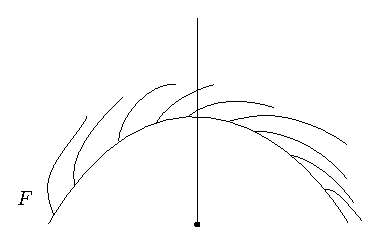
\includegraphics[width=0.35\textwidth]{MA4L8_1.eps}
		\caption{Невозможность причесать ежа.}
		\label{8_1}
	\end{figure}
\end{rem}
\textbf{Пример касательного векторного поля}: Рассмотрим $S^1$, тогда касательным векторным полем можно рассматривать: $V(x) = (x_2, -x_1) \Rightarrow$ если посчитать его в точках сферы, то $\inner{x}{V(x)} = 0$. 

\begin{proof}
	(От противного) Пусть $V(x) \neq 0$ на $S^{2n} \Rightarrow V(x) \neq 0$ в окрестности $S^{2n}$, тогда рассмотрим новое векторное поле, получаемое нормировкой:
	$$
		W(x) = \dfrac{V(x)}{\|V(x)\|} \colon \MR^{2n+1} \to\MR^{2n+1}
	$$
	это гладкое в окрестности $S^{2n}$ отображение из $\MR^{2n+1}$ в $\MR^{2n+1}$. Рассмотрим функцию:
	$$
		g(x) = \|x\|{\cdot}W\left(\tfrac{x}{\|x\|}\right)
	$$
	это гладкая функция на $\MR^{2n+1} \setminus \{0\}$ (можно доопределить до непрерывной в нуле). Рассмотрим функцию:
	$$
		F_t(x) = x + tg(x),\, t \in [0,1]
	$$
	для каждого $t$ это гладкая функция в окрестности $S^{2n}$. Рассмотрим множество:
	$$
		V_{a,b} = \{x \colon a < \|x\| < b\}, \, 0 < a < b < 1
	$$
	это есть ничто иное, как сферический слой. 
	\begin{figure}[H]
		\centering
		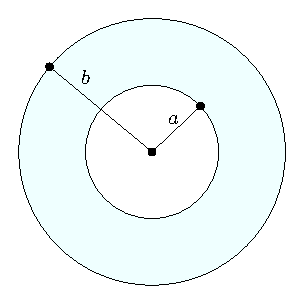
\includegraphics[width=0.2\textwidth]{MA4L8_2.eps}
		\caption{Сферический слой.}
		\label{8_2}
	\end{figure}
	Пусть верно: $0 < a_1 < a < b < b_1 < 1$, тогда $\exists \, t_0 \colon \forall t \in [0,t_0]$ такое, что выполнены два пункта:
	\begin{enumerate}[label=\arabic*)]
		\item $F_t$ на $\ovl{V}_{a_1,b_1}$ - инъекция (по аналогии с теоремой Брауэра):
		$$
			\forall x,z \in \ovl{V}_{a_1,b_1} \colon \|F_t(x) - F_t(z)\| \geq \|x - z\| - t\|g(x) - g(z)\| \geq (1 - t{\cdot}L)\|x - z\|
		$$
		где неравенство снова следует из гладкости $g$, далее выбираем $t$ так, чтобы последнее выражение было полжительным $\Rightarrow$ получаем инъективность;
		\item $\det{(F'_t)} > 0$ на $\ovl{V}_{a_1,b_1}$ (по аналогии с теоремой Брауэра): $(t,x) \to \det{(F'_t(x))}$ - непрерывна на $\ovl{V}_{a_1,b_1} \Rightarrow$ равномерно непрерывна, $\det(F'_0(x)) = 1 \Rightarrow$ по аналогии $\exists \, t_0$, когда $\det(F'_{t_0}(x)) > \frac{1}{2}$;
	\end{enumerate}
	Тогда, $F_t(V_{a_1,b_1})$ - открытое множество и $F_t \colon V_{a_1,b_1} \to F_t(V_{a_1,b_1})$ - диффеоморфизм (проверка такая же, как в теореме Брауэра). Рассмотрим образ кольца: $F_t(V_{a,b})$, чтобы понять что это мы рассмотрим образ сферы, радиуса $r \colon a < r < b$: $\{x \colon \|x\| =r \} = S_r$. Заметим, что:
	$$
		\inner{x}{V(x)} = 0 \Rightarrow \inner{x}{W(x)} = 0 \Rightarrow \inner{x}{g(x)} = 0
	$$ 
	следовательно $x$ и $tg(x)$ - перпендикулярны $\Rightarrow$ по теореме Пифгора будет верно:
	$$
		\|x \| =r \Rightarrow \|F_t(x)\|^2  = \|x\|^2 + t^2{\cdot}\|g(x)\|^2 = r^2 + t^2{\cdot}\|x\|^2 = (1 + t^2)r^2 \Rightarrow F_t(S_r) \subset S_{r\sqrt{1 + t^2}}
	$$
	$F_t$ это диффеоморфизм $\Rightarrow$ образ компакта - компакт $\Rightarrow F_t(S_r)$ это компакт, в частности, это замкнутое множество в $S_{r\sqrt{1 + t^2}}$. С другой стороны: $F_t(S_r)$ это открытое множество в $S_{r\sqrt{1 + t^2}}$: пусть мы взяли некоторую точку $a \in S_r$, рассмотрим её образ $F_t(a)$, поскольку $F_t$ это диффеоморфизм, то существует окрестность точки $a$ в $\MR^{2n+1}$ и окрестность точки $F_t(a)$ в $\MR^{2n+1}$ между которыми $F_t$ осуществляет диффеоморфизм.
	\begin{figure}[H]
		\centering
		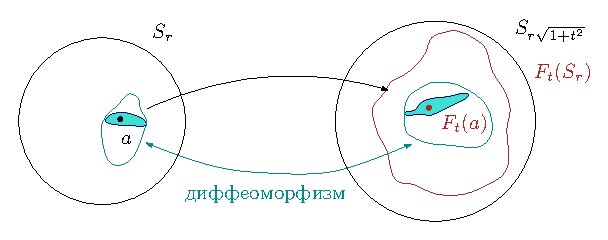
\includegraphics[width=0.65\textwidth]{MA4L8_3.eps}
		\caption{Диффеоморфизм.}
		\label{8_3}
	\end{figure}
	Поскольку диффеоморфизм переводит внутренние точки во внутренние, внешние во внешние, то пересечения этих окрестностей со сферами переходят друг в друга. Но пересечение открытого множества со сферой это и есть открытое множество на этой сфере $\Rightarrow$ в образе, $F_t(a)$ лежит с некоторой окрестностью.
	Сфера связное множество, тогда: 
	$$
		F_t(S_r) = S_{r\sqrt{1 + t^2}} \Rightarrow F_t(V_{a,b}) = V_{\sqrt{1+ t^2}a, \sqrt{1 + t^2}b}
	$$ 
	При маленьких $t$, используем ФЗП:
	$$
		|V_{\sqrt{1+ t^2}a, \sqrt{1 + t^2}b}| = (1 + t^2)^{\tfrac{2n + 1}{2} }{\cdot}|V_{a,b}| = \ddint{V_{a,b}}{}\det{(F'_t(x))}dx = P(t)
	$$
	где последнее верно, так как $x \mapsto \sqrt{1 + t^2}x$ и мы снова получили многочлен от $t$, следовательно:
	$$
		(1 + t^2)^{\tfrac{2n + 1}{2} }{\cdot}c = P(t), \, c > 0
	$$
	Такого быть не может, поскольку слева будет $(1 + t^2)^n{\cdot}\sqrt{1 + t^2} = P(t) \Rightarrow$ поскольку всё от $t^2$, то понятно, что многочлен $P(t)$ - четная функция $\Rightarrow$ обозначим $s = 1 + t^2$, тогда:
	$$
		c{\cdot}s^{n + \tfrac{1}{2}} = \wte{P}(s)
	$$
	Это невозможно, поскольку справа многочлен после конечного числа дифференцирований будет равен нулю, а выражение слева после любого числа дифференцирования не ноль, поскольку степень - дробная $\Rightarrow$ мы получили противоречие.
\end{proof}

\end{document}